% Very simple template for lab reports. Most common packages are already included.
\documentclass[a4paper, 11pt]{article}
\usepackage[utf8]{inputenc} % Change according your file encoding
\usepackage{graphicx}
\usepackage{url}
\usepackage{fancyvrb}

%opening
\title{Chordy - a distributed hash table}
\author{Chrysoula Dikonimaki}
\date{\today{}}

\begin{document}

\maketitle

\section{Introduction}
The goal of this exercise was to implement Chordy, a distributed hash table. The nodes are placed in a ring. Each node has a unique key and a store with  key-value pairs for which it is responsible. The store contains all the keys in the range (Pkey, Id], where Pkey is its Predecessor's key.

\subsection{Debugging message}
I added a new message called 'info' for debugging purposes. When a node receives a message like this it prints the most important information: the predecessor, the successor, the store etc.

\section{Performance}
\subsection{Experiment 1}
The function called run1() creates 1000 messages that will be added to the ring and 1000 messages that won't added. The rings contains 4 nodes. I looked up for 4000 messages asking the first node added to the ring. Then I looked up for the same 4000 messages but asking 4 different nodes giving to each one of them 1000 messages. I ran the experiment twice and the results are shown in Figure \ref{exp1}. In general, the time will depend on how the keys are distributed.

\begin{figure}
  \begin{center}
    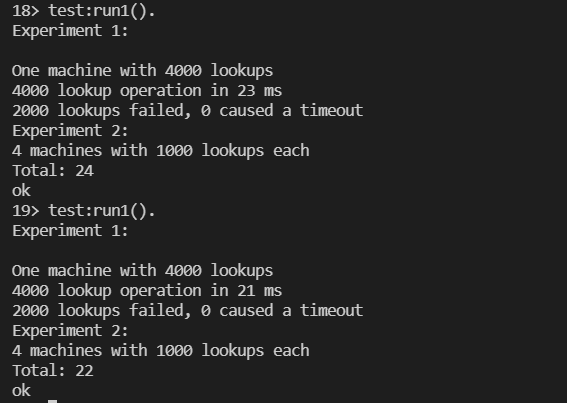
\includegraphics[scale=0.4]{exp1.PNG}
    \caption{Running the first experiment twice}
    \label{exp1}
  \end{center}
\end{figure}

\subsection{Experiment 2}
The results of the second experiments are shown in Table \ref{table:1}. I ran the function run2 setting the parameters shown in the table. It is obvious, that when we increase the number of Nodes the time increases.

\begin{table}[h!]
\centering
\begin{tabular}{ c c }
 Number of Nodes & Time (in ms)  \\ 
 \hline
 100 & 3  \\  
 101 & 3 \\
 1000 & 16 \\
 10000 & 594 \\
 100000 & 919
\end{tabular}
\caption{Experiment 2: number of pairs =  100}
\label{table:1}
\end{table}

\section{Handling Failures}
We should detect and handle failures by monitoring each node's successor and predecessor. When the predecessor dies it will be handled automatically but when the successor dies our new successor is the previous successor's successor. That's why we have to save the next node. If we wanted to handle many failures at the same time, we could have a list with the next nodes, but it would be inefficient.

I created 3 nodes (X, Y, Z) and then I stopped Y. Figure \ref{exp2_1} shows the information for each node before Y stops and figure \ref{exp2_2} shows the same information for X and Y after Y died.
\begin{figure}
  \begin{center}
    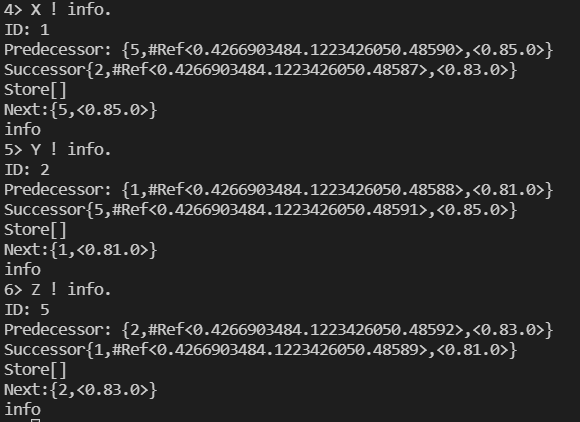
\includegraphics[scale=0.4]{exp2_1.PNG}
    \caption{}
    \label{exp2_1}
  \end{center}
\end{figure}

\begin{figure}
  \begin{center}
    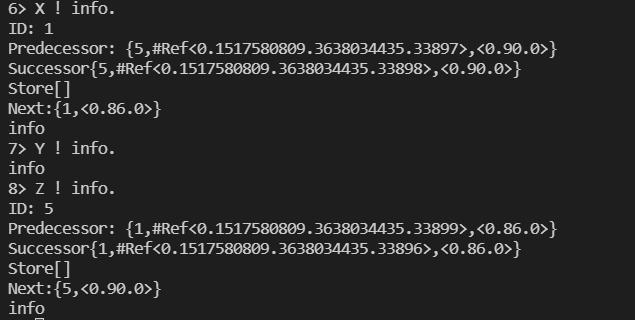
\includegraphics[scale=0.4]{exp2_2.PNG}
    \caption{}
    \label{exp2_2}
  \end{center}
\end{figure}

\section{Replication}
Saving the replicas at the successor is a good idea because if a node crash its pairs will be at the right place and we won't do something special to get them to its successor. However, there is always a chance to crash both the node and its successor at the same time and data won't be found anywhere.

Figure \ref{exp3_1} shows the information about 3 nodes (X, Y and Z). Y has the values a and b while Z has the value c. In Figure \ref{exp3_2} we can see the information of X and Z after stopping the node Y. We can see that everything works correctly.
\begin{figure}
  \begin{center}
    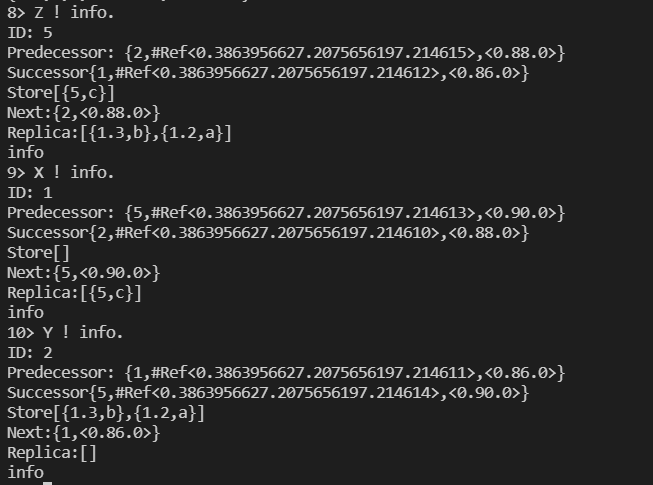
\includegraphics[scale=0.4]{exp3_1.PNG}
    \caption{}
    \label{exp3_1}
  \end{center}
\end{figure}

\begin{figure}
  \begin{center}
    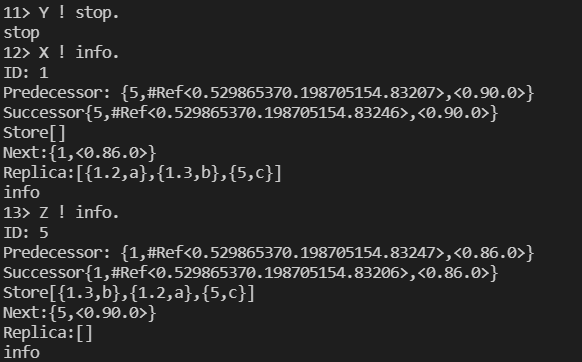
\includegraphics[scale=0.4]{exp3_2.PNG}
    \caption{}
    \label{exp3_2}
  \end{center}
\end{figure}

\section{Conclusions}
Building a hash table is not that hard, but we have to think a lot about the possible failures and ways to handle them. The advantage of having a distributed store is the fault tolerance that it provides because even if the node fails its values will be saved somewhere and they won't get lost. However, storing data remotely has the overhead of transferring all these data over the network and maintain redundant copies. Things can get really hard if we want to modify the values because we will need to keep the copies updated as well.
\end{document}
